% add figures from the VC paper
\chapter{Methodology}\label{ch:4}

\section{Proposed Framework}
Reviewing a variety of regional revitalization cases, we sketched a diagram at Figure 4.1 to summarize their common mechanism.
In a common case of regional revitalization, the authority makes use of local specialties and applies new ideas with technology to improve existing industry or establish a new one,
usually a tourism business, which succeeds to attract more people to visit the place and activate local economy.

We also sketched a diagram at Figure 4.2 to describe a common mechanism of regional revitalization that implements location-based AR.
In such cases, the authority applies new ideas on local features to compose unique contents for a location-based AR service,
which motivates people to access the place more, resulting in an improvement in local economy.
Despite that the contents are in digital form or accessible online, the system's location-based characteristics still make it to encourage visitors to access physically.

\begin{figure}
  \begin{minipage}{0.48\textwidth}
    \centering
    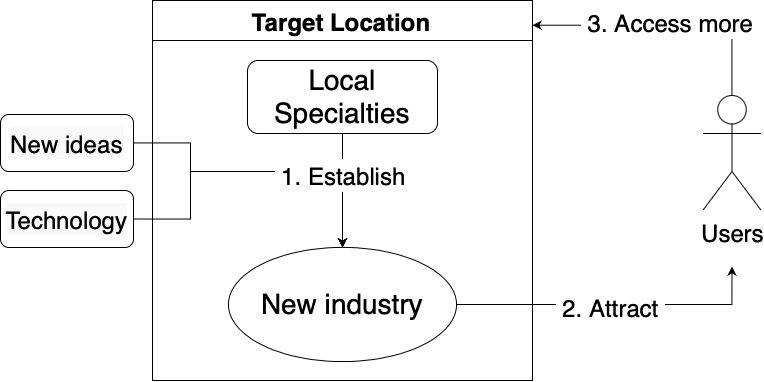
\includegraphics[width=0.9\linewidth]{resources/4_methodology/common_vitalization.png}
      \caption{Common framework of Regional Revitalization}
  \end{minipage}\hfill
  \begin{minipage}{0.48\textwidth}
    \centering
    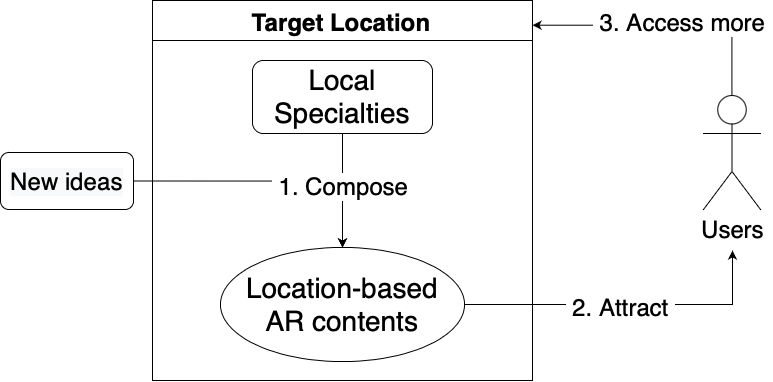
\includegraphics[width=0.9\linewidth]{resources/4_methodology/revitalization_with_AR.png}
      \caption{Framework of Regional Revitalization with location-based AR}
  \end{minipage}
\end{figure}

For places like public facilities where there is a lack of local features usable to attract visitors,
we presented a framework, sketched in Figure 4.3, that adopts a common characteristic of the places: users.
In our assumption, by enabling users to engage in co-creation of contents, which can be conducted digitally with low costs in a location-based AR system,
we anticipate that the problem of lacking usable resources becomes solvable.
Besides the issue of content creation, From Section 3.1, 3.2 and 3.3 we understand the influence on users' motivation and images about a place by both location-based AR and co-creation,
which are both included in our framework.
We also introduce a socializing mechanism to encourage users to participate in the co-creation process.
From Section 3.4 we understand that interaction between users improves people's engagement with a co-creation activity.

For this framework we proposed, we developed a prototype according to the idea of the framework, and later we examined the proposed framework with an experiment with the prototype.

\begin{figure}
  \centering
  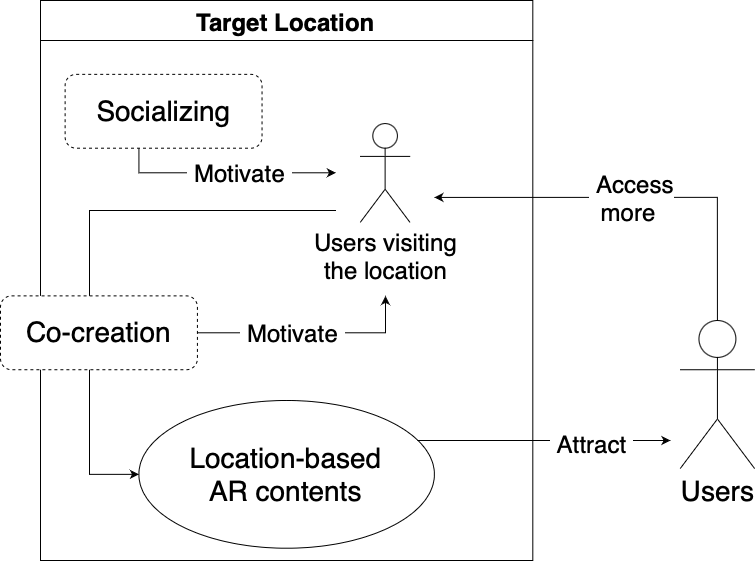
\includegraphics[width=0.8\columnwidth]{resources/4_methodology/revitalization_with_AR_and_cocreation.png}
    \caption{Proposed framework: Revitalization with location-based AR and Co-creation}
\end{figure}

\section{Prototype}
The prototype is a Web AR mobile app, where users paint their own virtual graffiti, view other users' graffiti, and create graffiti based on other users' ones around Nishi-Waseda Campus of Waseda University.
We deployed the app on web instead of publishing a native app, so that users with a mobile device of any brand can easily access the service on their web browsers.
The front-end part is built with ReactJS (Javascript), and the back-end part, handling authentication, database and storage, is served by Google Firebase.
The functionality of location-based AR is implemented with AR.js, A-Frame and Javascript Geolocation API.

The prototype was supposed to enable creating graffiti at any place in the campus, but due to the consideration of unsufficient GPS accuracy and security issues,
we restricted the places where graffiti are visible to several specific locations at campus.
In Figure 4.4, the prototype displays pins on the specific locations. The device's GPS information is retrieved to confirm where the user is.
When a user gets close enough to one of the pinned locations, the corresponding pin turns yellow to indicate that the graffiti there is available to access.
In Figure 4.5, when a pin is touched, a picture of the location is displayed so that the user can confirm the exact location and face to the correct orientation.

\begin{figure}
  \begin{minipage}{0.48\textwidth}
    \centering
    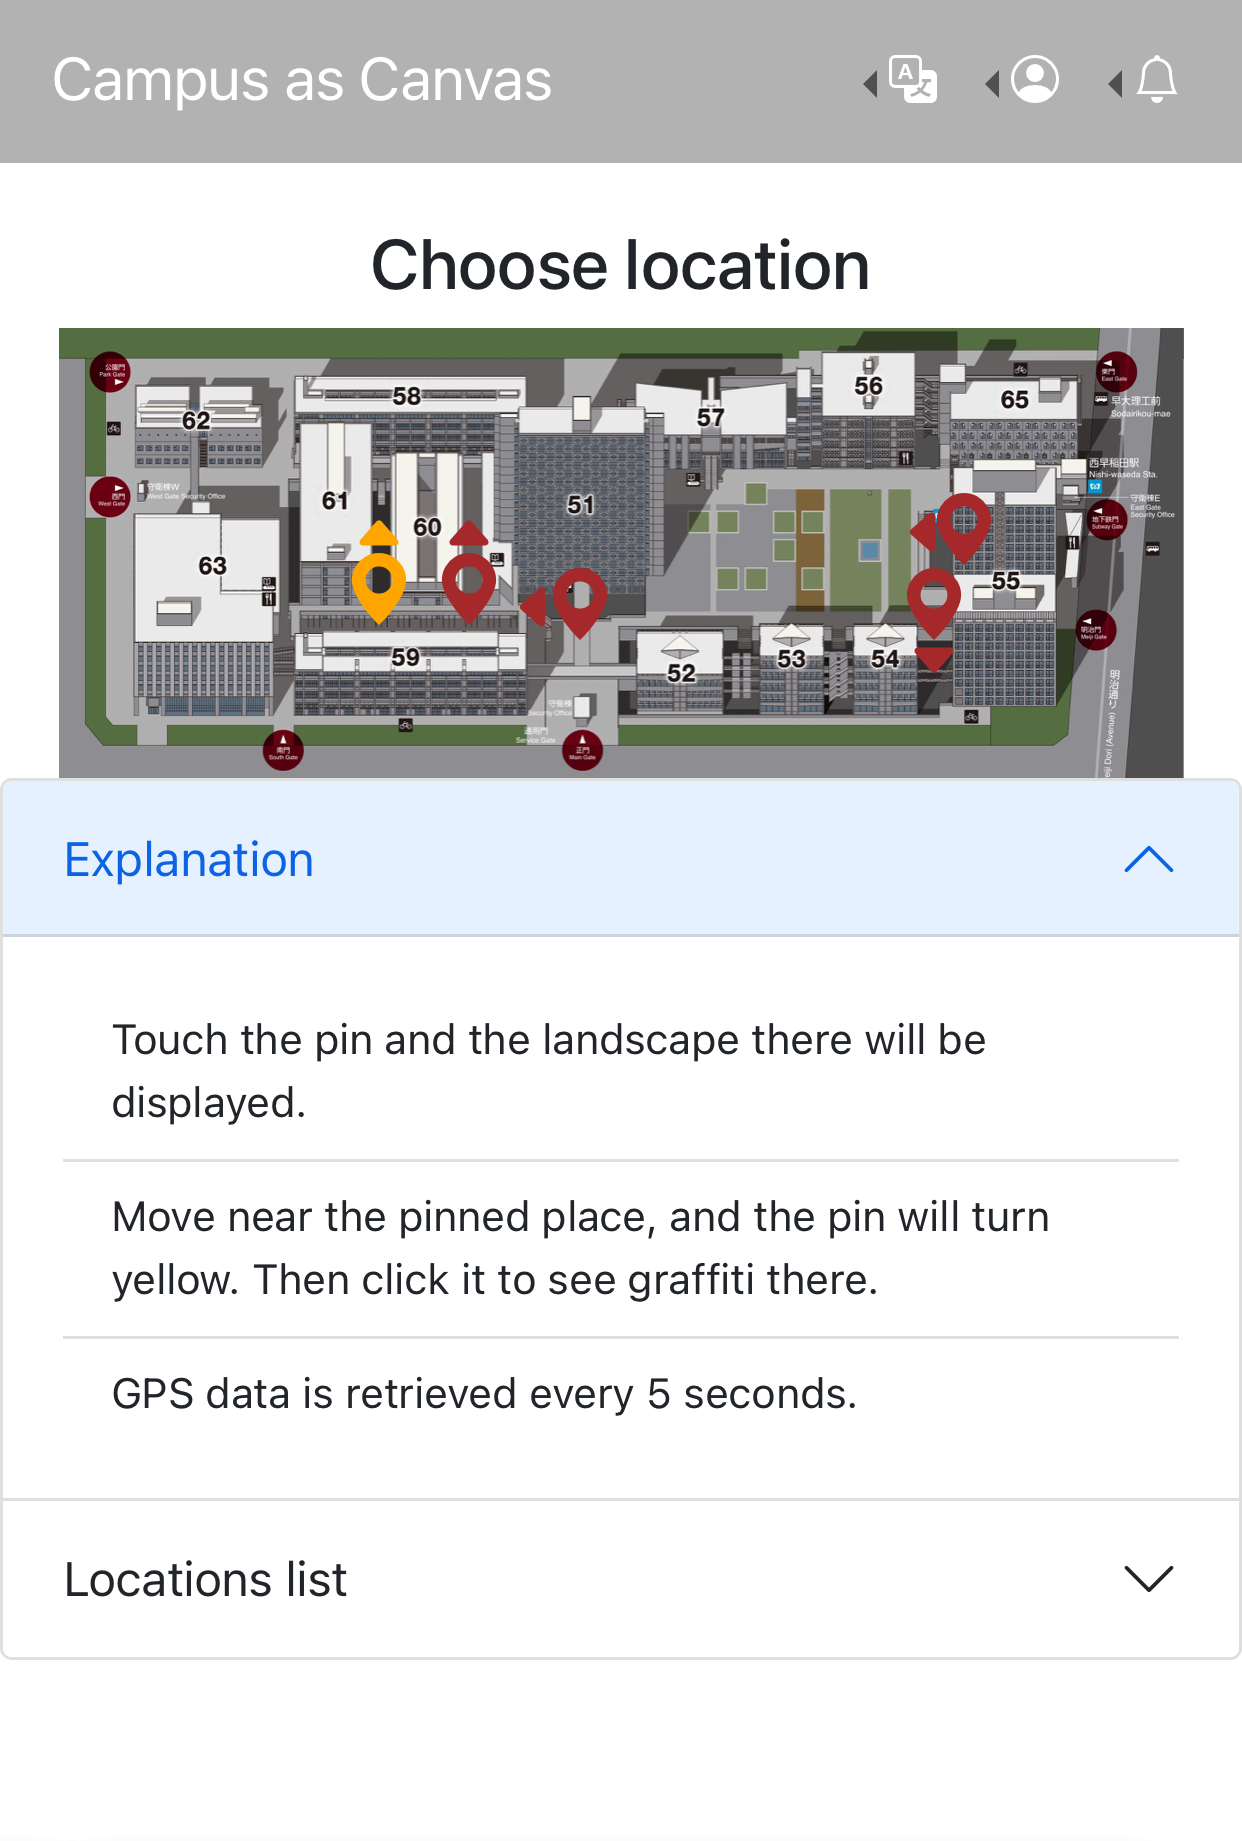
\includegraphics[width=0.9\linewidth]{resources/4_methodology/prototype_home.png}
      \caption{Prototype screenshot: Home page}
  \end{minipage}\hfill
  \begin{minipage}{0.48\textwidth}
    \centering
    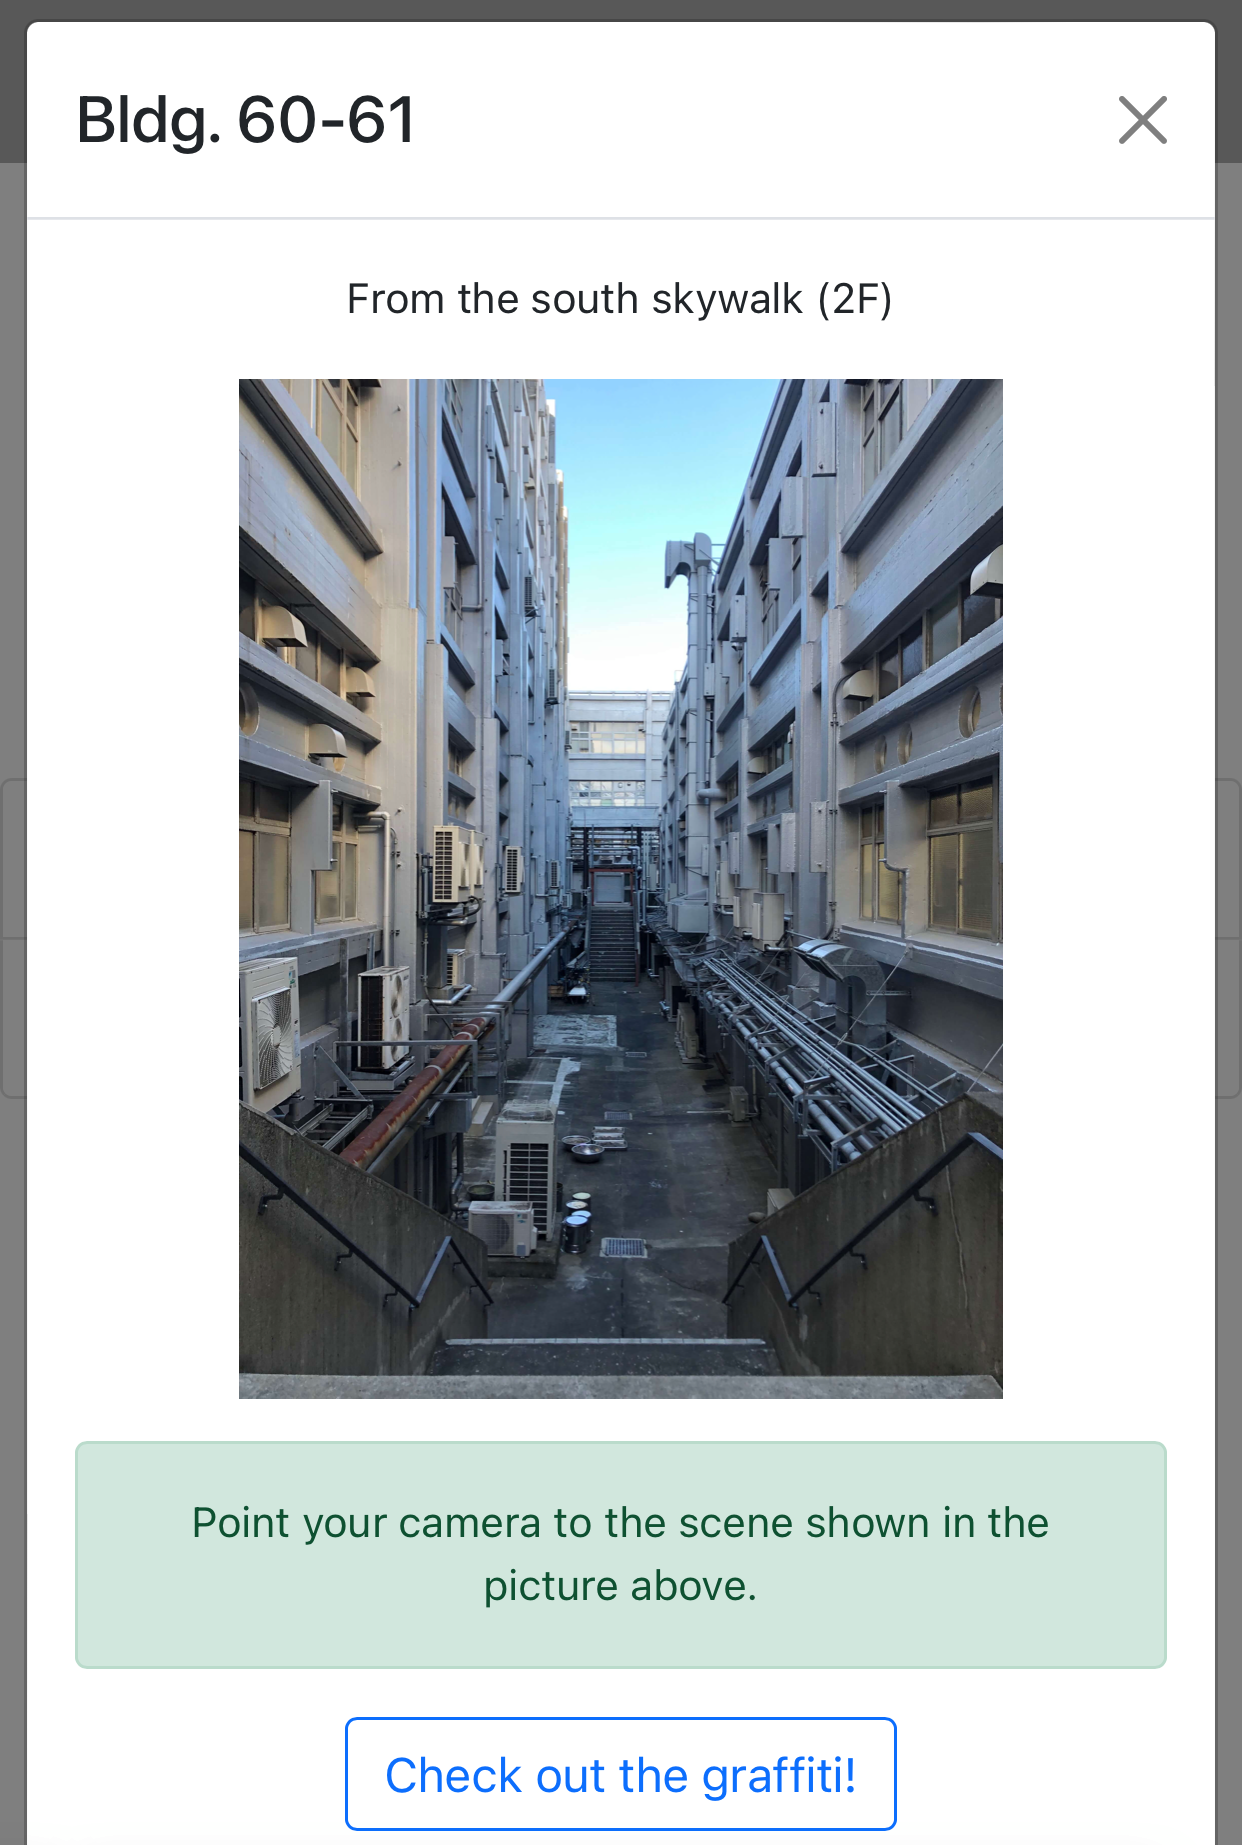
\includegraphics[width=0.9\linewidth]{resources/4_methodology/prototype_loc_pic.png}
      \caption{Prototype screenshot: Picture for confirming the location}
  \end{minipage}
\end{figure}

After confirming the location, the app switches to AR mode by turning on the camera, and graffiti are displayed with the real landscape as a background, as shown in Figure 4.6.
The menu on the bottom displays a graffiti's title, description, 'Like' button, button to check the same user's all creation, and a 'New!' button to open a painting canvas.
There are also buttons on the left and right to switch between different graffiti.
For graffiti painted based on other ones, as shown in Figure 4.7, there is a 'Based works' button to display the previous graffiti which this one is based on.

\begin{figure}
  \begin{minipage}{0.48\textwidth}
    \centering
    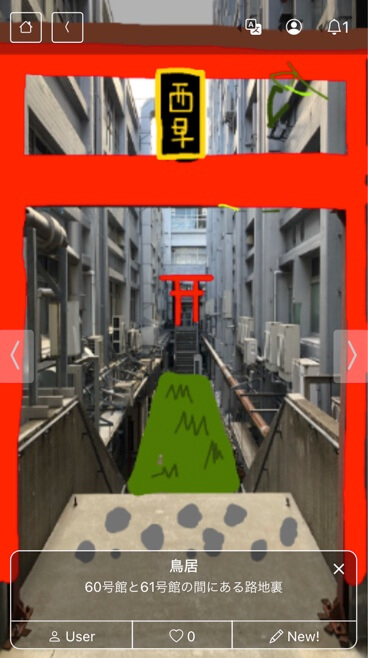
\includegraphics[width=0.9\linewidth]{resources/4_methodology/prototype_graffiti.png}
      \caption{Prototype screenshot: Graffiti displayed in AR mode}
  \end{minipage}\hfill
  \begin{minipage}{0.48\textwidth}
    \centering
    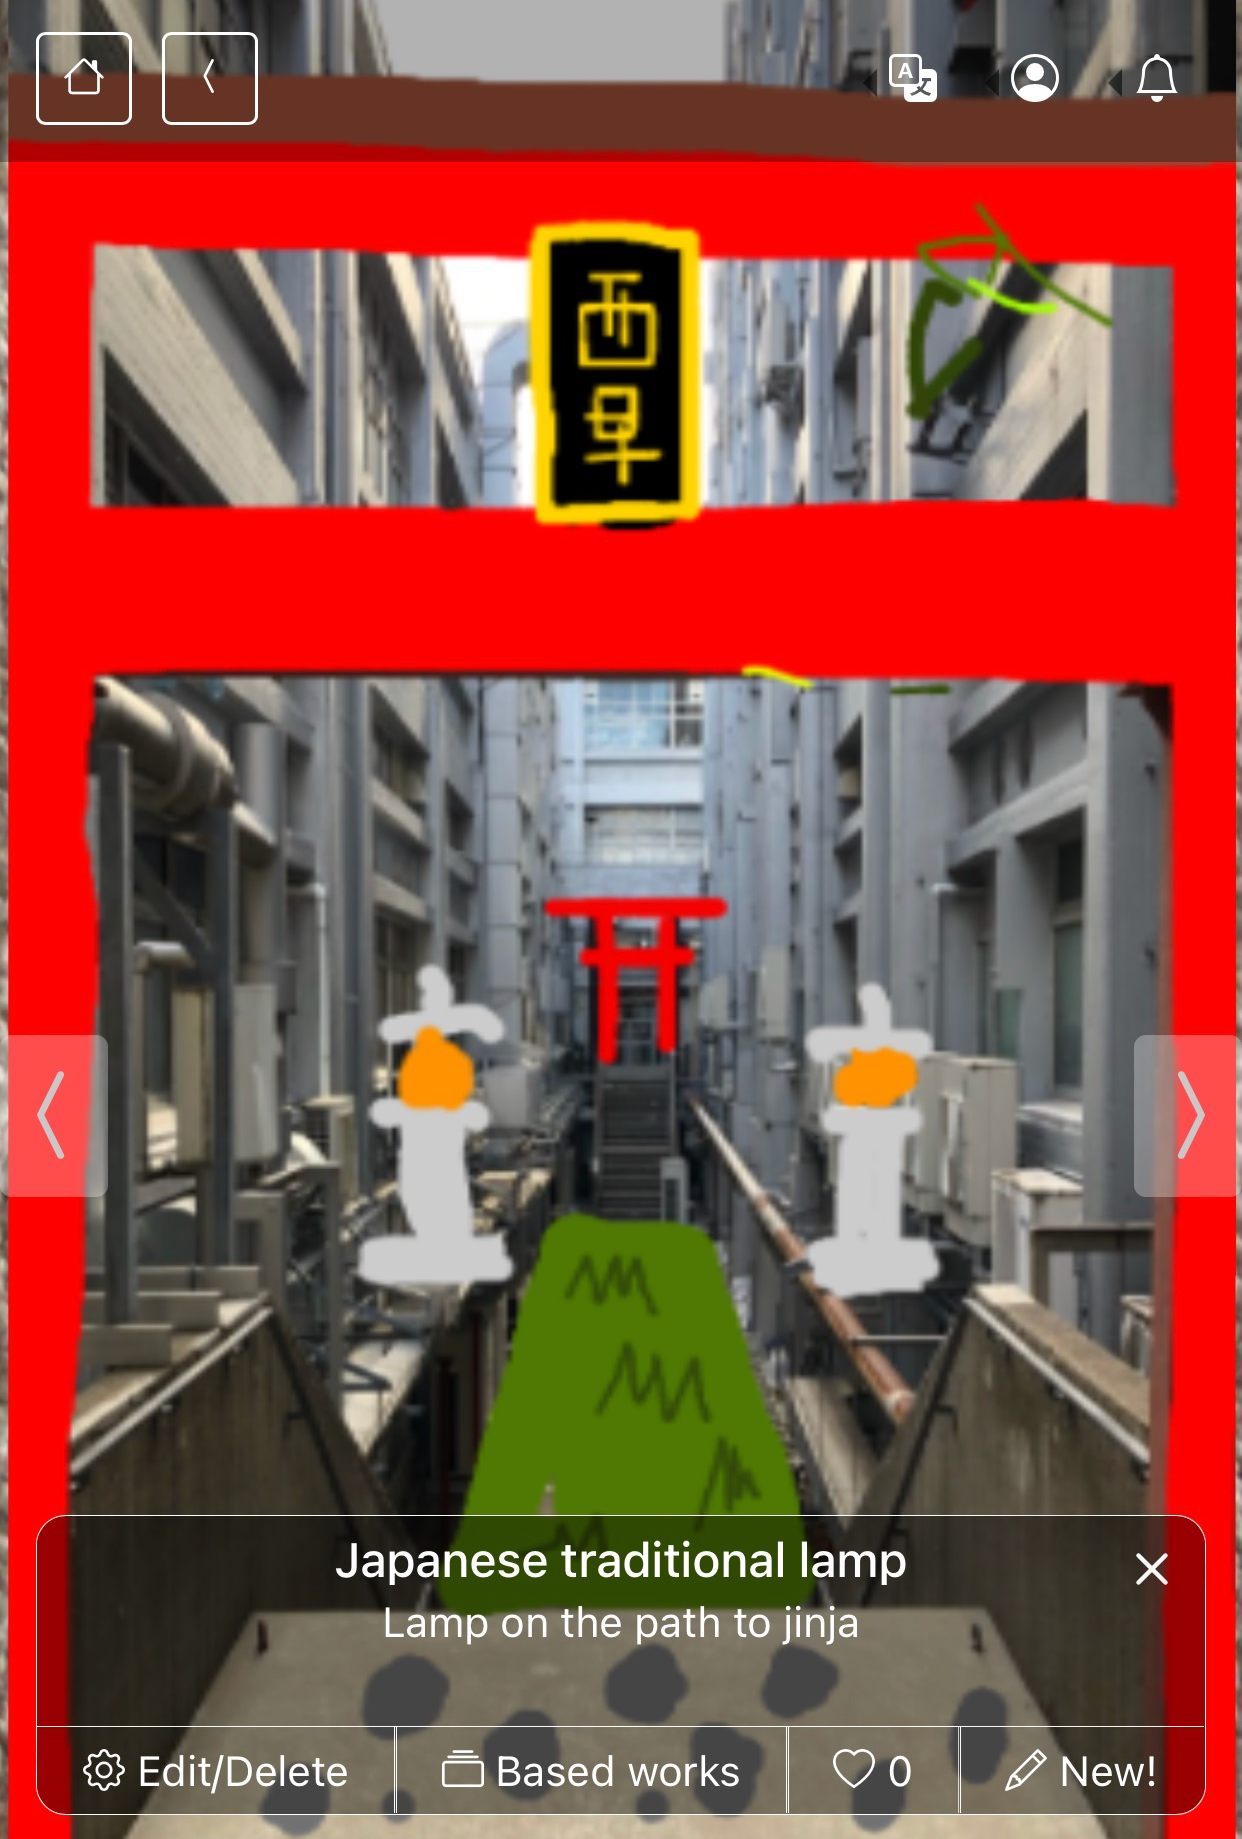
\includegraphics[width=0.9\linewidth]{resources/4_methodology/prototype_based_graffiti.png}
      \caption{Prototype screenshot: A graffiti painted based on other ones}
  \end{minipage}
\end{figure}

With the features of A-Frame, each graffiti is located on its specific angle, recorded during creation, to fit the background landscape, as demonstrated in Figure 4.8.

\begin{figure}
  \centering
  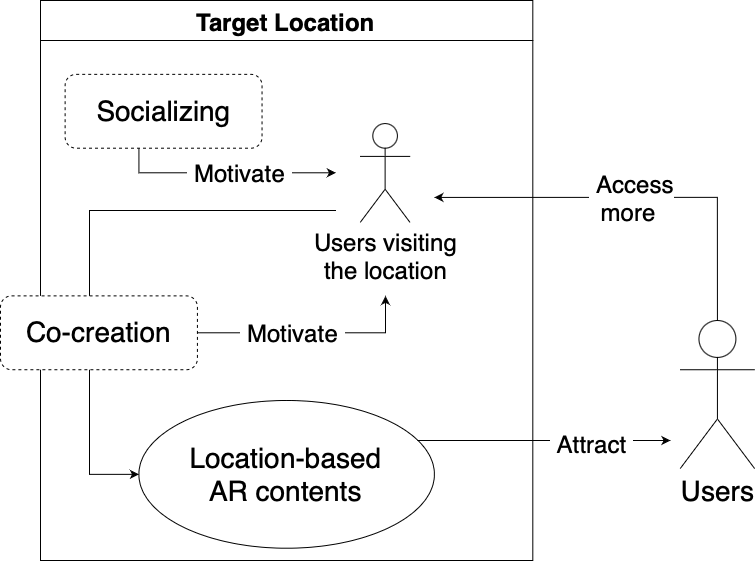
\includegraphics[width=0.8\columnwidth]{resources/4_methodology/revitalization_with_AR_and_cocreation.png}
    \caption{Prototype screenshot: Graffiti displayment in different angles to fit itself to the landscape}
\end{figure}

On clicking the 'New!' button, as shown in Figure 4.9, the user can choose between creating a new graffiti and painting on another user's graffiti,
and then a canvas is expanded with basic painting tools equipped, as shown in Figure 4.9.
Last but not least, whenever a graffiti is 'liked' or someone painted another graffiti based on this one, the author receives notifications in the app.

\begin{figure}
  \begin{minipage}{0.48\textwidth}
    \centering
    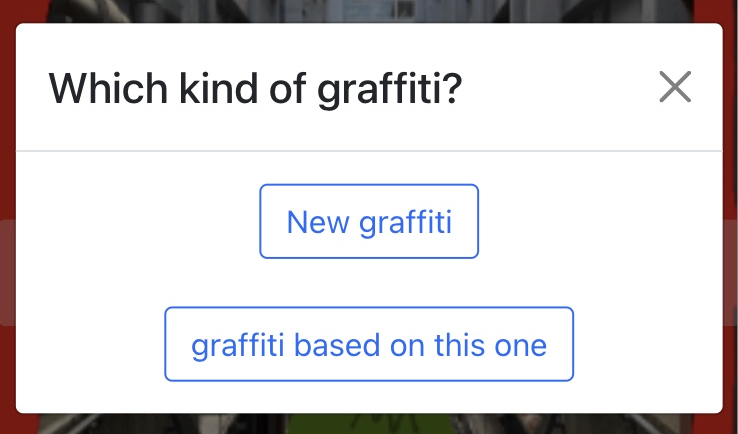
\includegraphics[width=0.9\linewidth]{resources/4_methodology/prototype_choose_graffiti_type.png}
      \caption{Prototype screenshot: Menu for choosing the type of graffiti painting}
  \end{minipage}\hfill
  \begin{minipage}{0.48\textwidth}
    \centering
    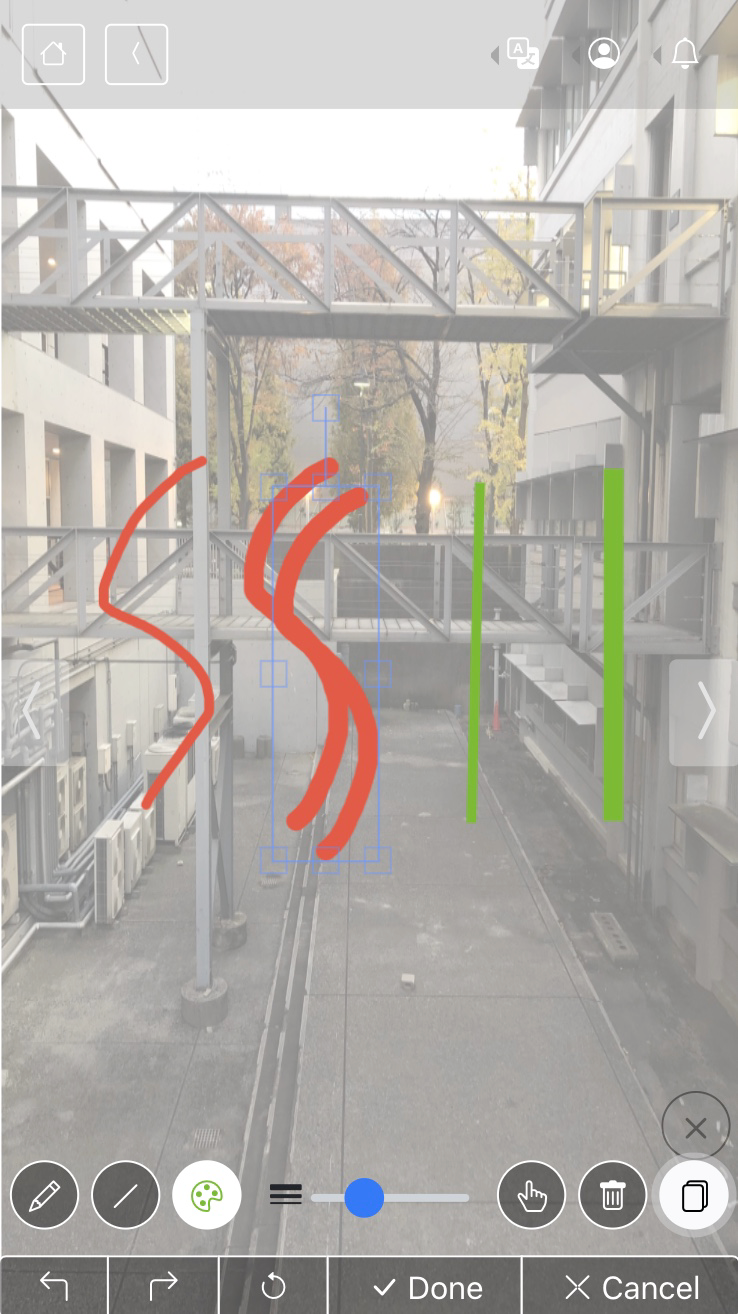
\includegraphics[width=0.9\linewidth]{resources/4_methodology/prototype_canvas.png}
      \caption{Prototype screenshot: Canvas and tools for graffiti painting}
  \end{minipage}
\end{figure}

In the prototype, content co-creation is realized by graffiti painting only by users,
and user-user interaction is implemented by functionalities of 'like' and painting basd on other users' graffiti.
